\chapter{DUNE Far Site Technical Coordination}
\label{ch:exec-tc}

\textit{This chapter provides a brief introduction to the DUNE far site technical coordination.  The text below closely follows that found in the introductory chapters of Volume~\volnumbertc{}, \voltitletc{}, where many more details may be found.}

%%%%%%%%%%%%%%%%%%%%%%%%%%%%%%%%%%%%%%%%%%%%%
\section{Overview}

Far site \dword{tc} concerns the organization and management of 
activities required to design, construct,
fabricate, install, and commission the \dword{dune} \dword{fd} modules properly and safely. 
      The \dword{dune} collaboration has direct responsibility for the design 
and construction of the \dword{dune} detectors.  Groups of collaborating 
institutions, referred to as consortia, assume responsibility for 
the different detector subsystems.  The activities of the consortia are 
overseen and coordinated through the \dword{dune} \dword{tc} organization 
headed by the \dword{dune} \dword{tcoord}.  The \dword{tc} organization 
provides project support functions such as safety coordination, 
engineering integration, change control, document management, scheduling, 
risk management, and technical review planning.  \dword{dune} \dword{tc} 
manages internal, subsystem-to-subsystem interfaces and ensures the proper integration of the different subsystems.   
%\fixme{instead of DUNE TCN above, should we say ``far site TCN'' as in first sentence?}

\dword{dune} \dword{tc} works closely with the support teams of its 
\dword{lbnf-dune} partners within the framework of a \dword{jpo} to 
ensure that project support functions across the entire global 
enterprise are coherent.  For consistency of the \dword{dune} \dword{esh} 
and \dword{qa} programs with those across \dword{lbnf-dune}, the 
%\dword{lbnf-dune} \dword{esh} and \dword{qa} 
managers of these programs, who sit within 
the \dword{jpo}, are also embedded within the \dword{dune} \dword{tc} 
organization.  The \dword{jpo} establishes the global engineering
and documentation requirements for the \dword{dune} 
\dword{fd} construction project, manages external \dword{dune} detector 
interfaces with \dword{lbnf}, and oversees proper 
integration of the \dword{dune} detector elements within the facilities 
and supporting infrastructure.  




Detector integration and installation activities are supported by the 
\dword{dune} consortia, which maintain responsibility for ensuring 
proper installation and commissioning of their subsystems.  External 
\dword{dune} interfaces with the onsite integration and installation 
activities are managed through the \dword{jpo}.




%%%%%%%%%%%%%%%%%%%%%%%%%%%%%%%%%%%%%%%%%%%%%
\section{Global Project Organization}
\label{sec:exec-tc-partners}

\subsection{Global Project Partners}

The \dword{lbnf} project is responsible for providing both the
\dword{cf} and supporting infrastructure (cryostats and
cryogenics systems) that house the \dword{dune} \dword{fd}
modules.  The international \dword{dune}
collaboration under the direction of its management team is
responsible for the detector components.  The \dword{dune} \dword{fd}
construction project encompasses all activities required for designing
and fabricating the detector elements. % and incorporates contributionsfrom a number of international partners.  
The organization of the
global \dword{lbnf-dune}, which encompasses both project elements, is
shown in Figure~\ref{fig:DUNE_global}.
\begin{dunefigure}[Global project organization]{fig:DUNE_global}
  {\dword{lbnf-dune} organization.}
  \includegraphics[width=0.95\textwidth]{FS_Integration_OrgChart_notitle}
\end{dunefigure}

The overall
coordination of installation activities in the underground caverns 
is managed as a separate element of \dword{lbnf-dune} under the
responsibility of the \dword{ipd}, who is appointed by and reports
to the \dword{fnal} director.  To ensure coordination across
all elements of \dword{lbnf-dune}, the \dword{ipd} connects to both
the facilities and detector construction projects through ex-officio
positions on the \dword{lbnf} Project Management Board and
\dword{dune} \dword{exb}, respectively, %.  In carrying out these
%responsibilities, the \dword{ipd} 
and receives support from the \dword{sdsd},
a \dword{fnal} division established to 
provide the necessary supporting infrastructure for installation, commissioning, and operation 
of the \dword{dune} detector.
The \dword{dune} consortia maintain responsibility 
for the installation and commissioning of their detector subsystems
and %support these activities by providing dedicated personnel and
%equipment resources.  Likewise, 
and \dword{lbnf} retains responsibility
for the installation and commissioning of supporting infrastructure
items. 
%\subsection{EFIG}
Both provide dedicated resources to support their activities, and the high-level
coordination between the construction 
projects is coordinated by the \dword{efig}, described in Section~\ref{es:ch1:intl-org-resp}.    
The 
%global far site
 integration organization of the \dword{lbnf-dune} is shown in Figure~\ref{fig:fs-integration-org-chart}. 

\begin{dunefigure}[LBNF/DUNE far site integration organization]{fig:fs-integration-org-chart}
  {\dword{lbnf-dune} far site integration organization.}
  \includegraphics[width=0.99\textwidth]{FS_Integration_OrgChart_notitle} %DUNE_global}
\end{dunefigure}

\begin{dunefigure}[JPO functions]{fig:DUNE_jpo}
  {\dword{jpo} global support functions and teams}
  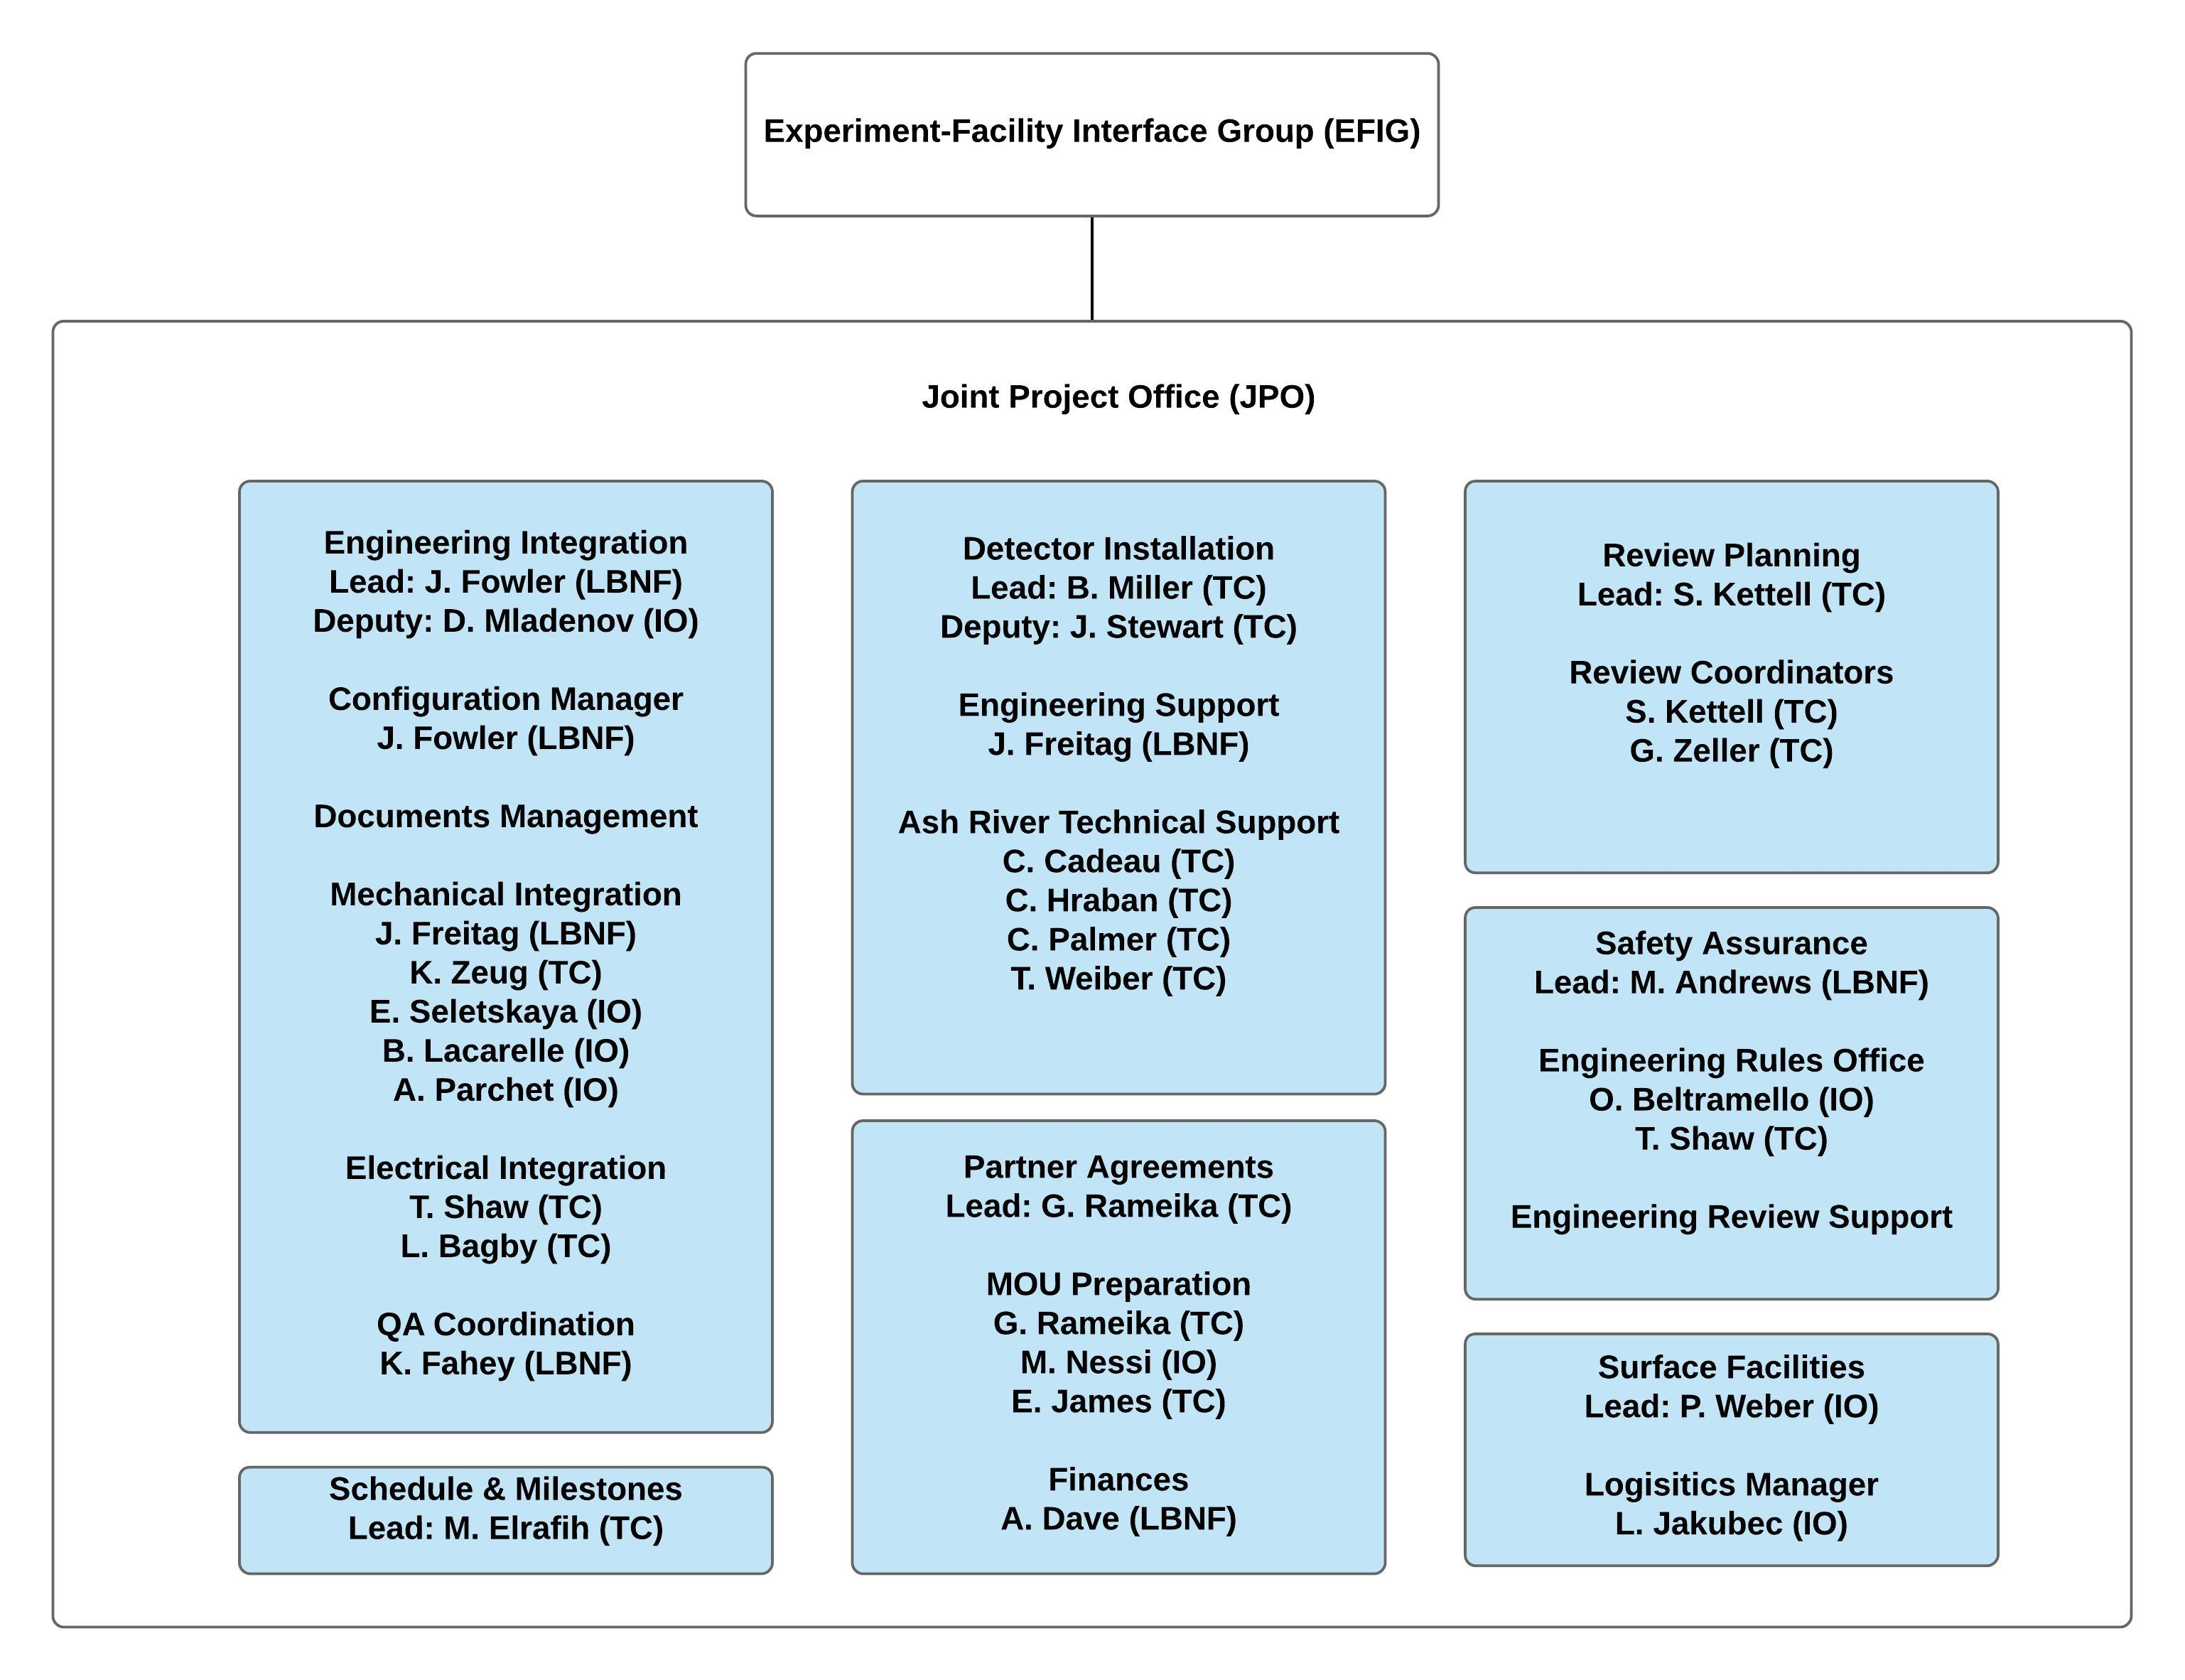
\includegraphics[width=0.85\textwidth]{JPO_OrgChart_v4}
\end{dunefigure}

%\subsection{JPO}
The \dword{efig} is augmented by the \dword{jpo}, which supports both 
the \dword{lbnf} and \dword{dune} projects as well as the integration
effort that connects the two together. The \dword{jpo} combines
project support functions that exist within the different elements 
of global project to ensure proper coordination across the entire 
\dword{lbnf-dune} enterprise.  Project functions coordinated globally 
through the \dword{jpo} are shown in Figure~\ref{fig:DUNE_jpo} along 
with the personnel currently supporting those functions.
%%
The \dword{jpo} organization will evolve over time to incorporate the 
onsite team responsible for coordinating integration and installation 
activities at \dword{surf} under the direction of the \dword{ipd}.  %%%

\begin{dunefigure}[JPO functions]{fig:DUNE_jpo}
  {\dword{jpo} global support functions and teams}
  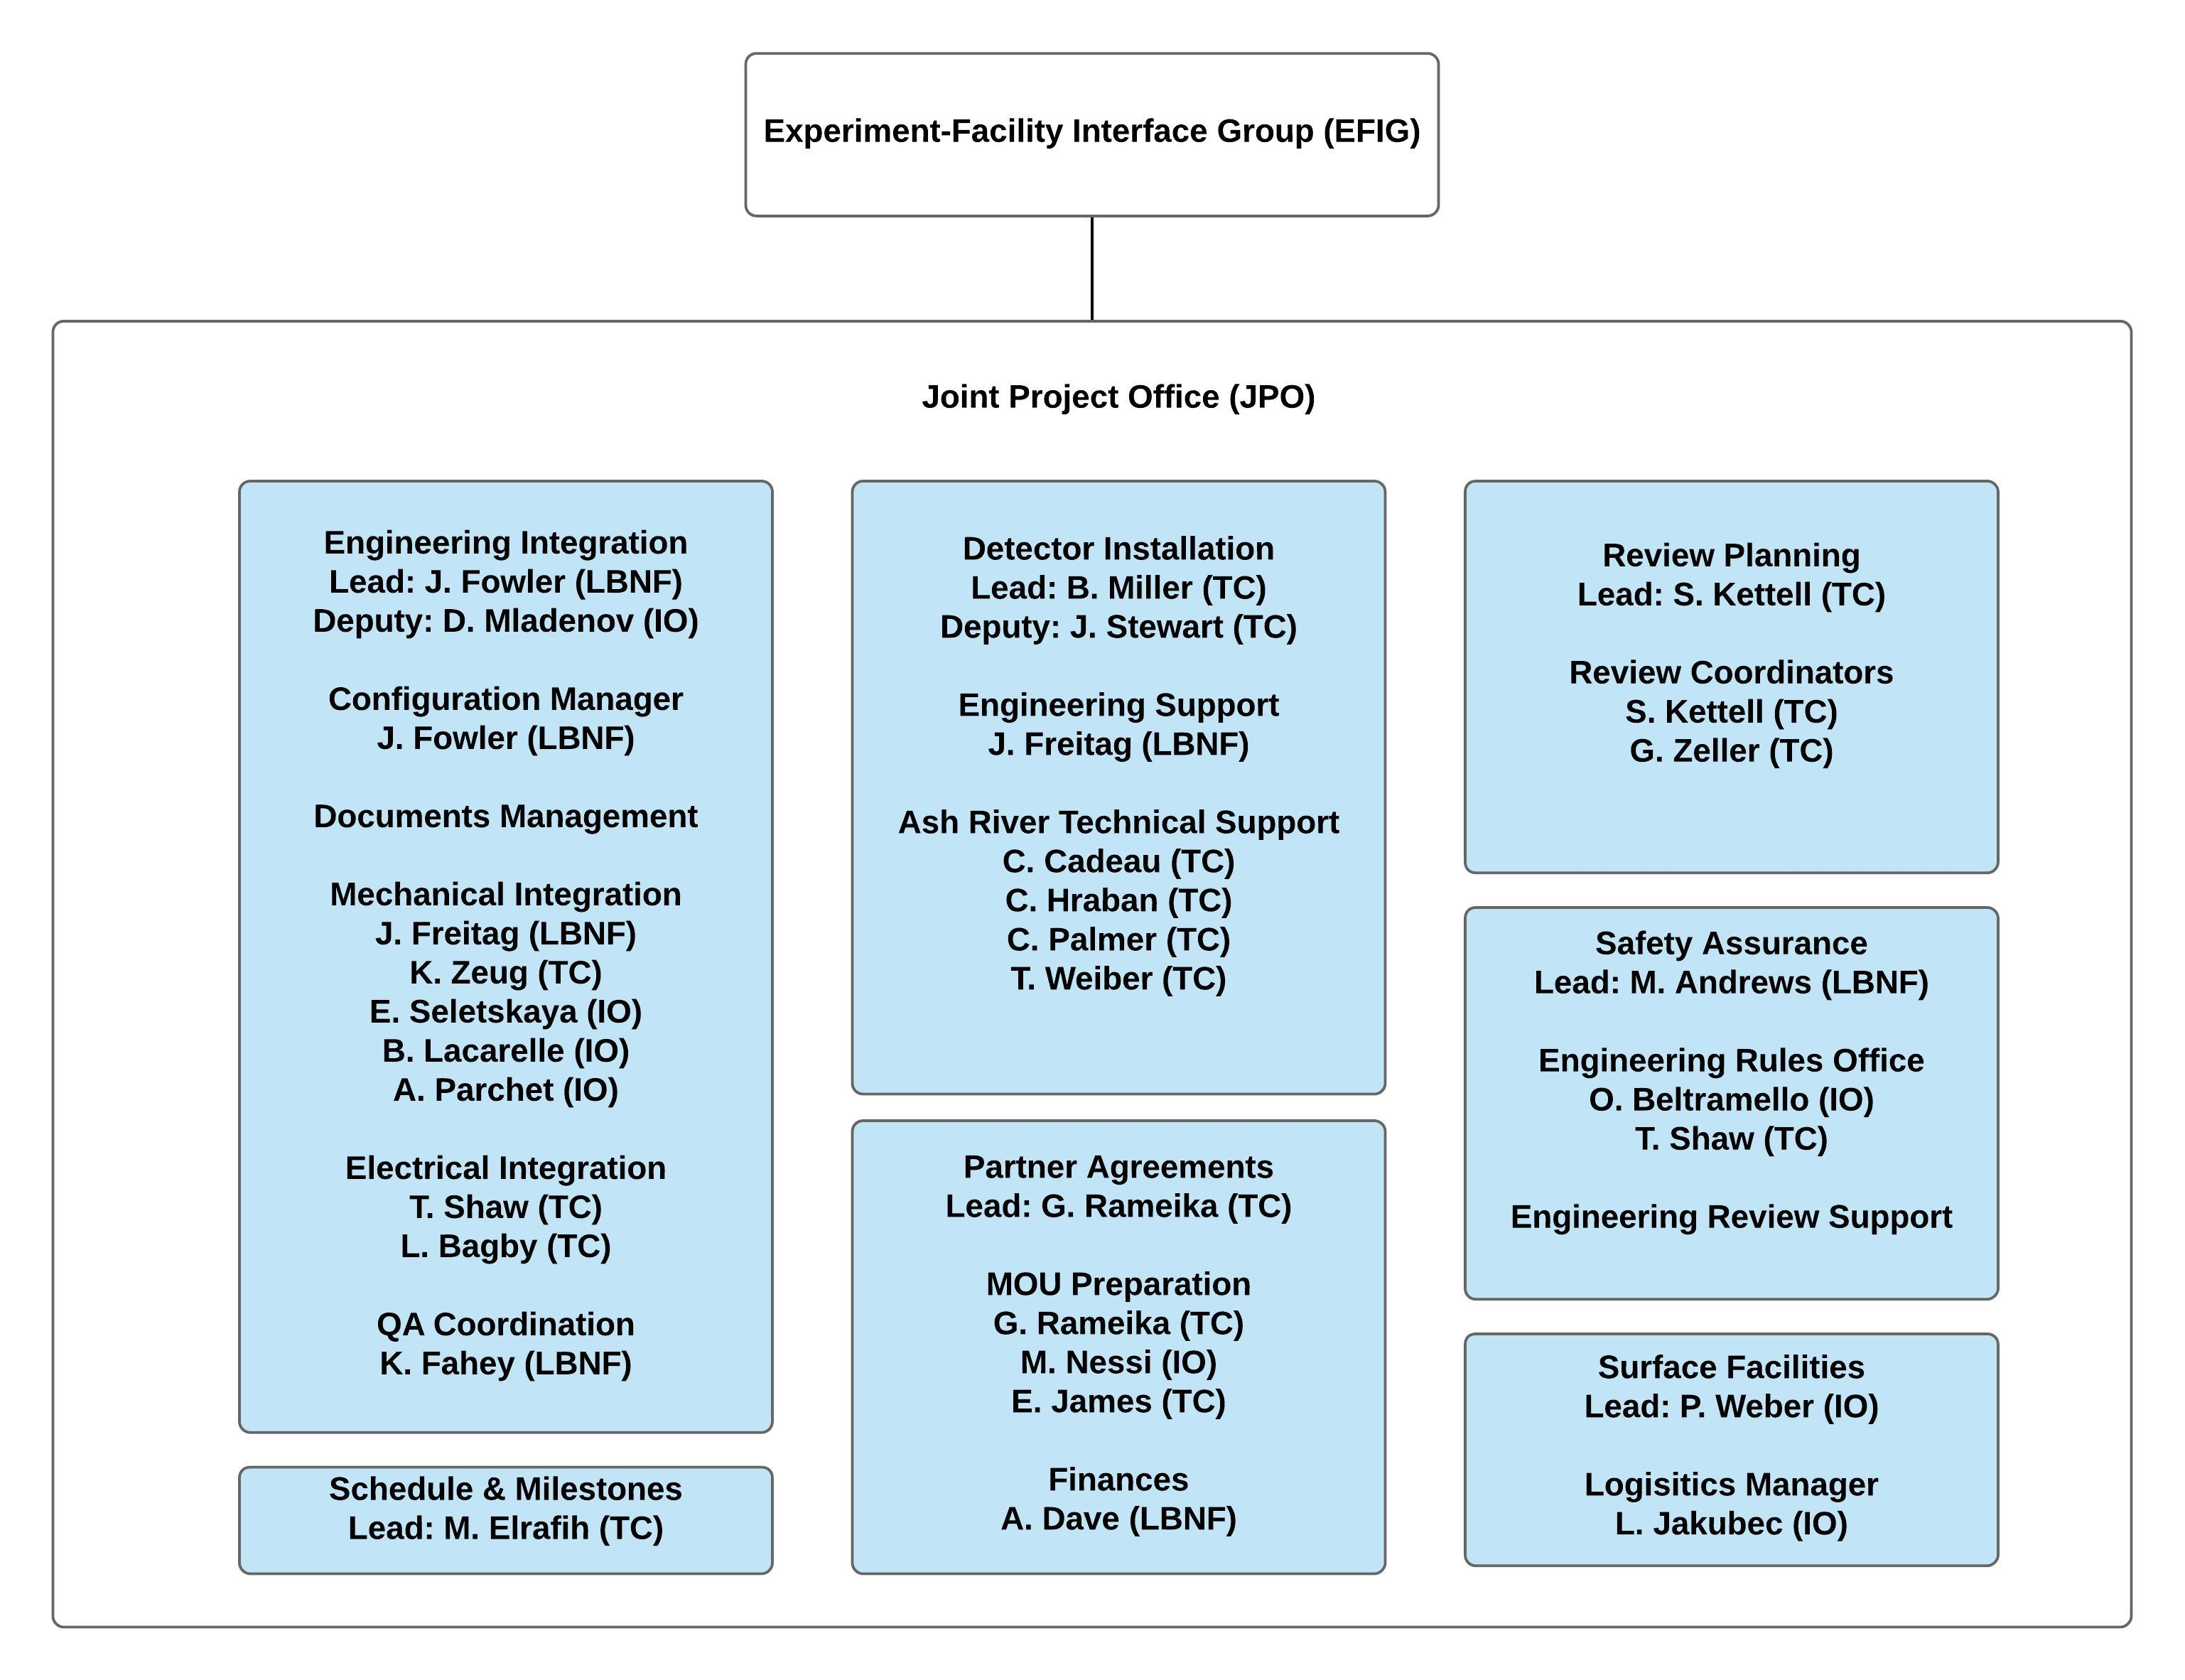
\includegraphics[width=0.85\textwidth]{JPO_OrgChart_v4}
\end{dunefigure}


\subsection{Coordinated Global Project Functions}

Project support functions requiring \dword{jpo} coordination include
safety, engineering integration, change control and document 
management, scheduling, review planning and oversight, and development 
of partner agreements.  

Planning activities related to detector installation and the provision 
of surface facilities are also currently embedded within the framework 
of the \dword{jpo} to ensure that all project elements are properly 
incorporated.  At the time when \dword{lbnf} \dword{fscf} delivers 
\dword{aup} of the underground detector caverns at \dword{surf}, the 
coordination of these activities will be fully embedded within 
a \dword{lbnf}/\dword{dune} \dword{integoff} under the direction of the \dword{ipd}. 

%%%

\subsection{Safety}
\label{sec:dune_safety}


For a consistent approach to safety across \dword{lbnf-dune},
a single project \dword{esh} manager reports  
to the \dword{lbnf} project director, \dword{ipd}, and \dword{dune}
management (via the \dword{dune} \dword{tcoord}).  This individual
directs separate safety teams responsible for implementing the
\dword{lbnf-dune} \dword{esh} program within both the \dword{lbnf} 
and \dword{dune} projects as well as the \dword{lbnf}/\dword{dune}
installation activities at \dword{surf}. The safety organization 
is shown in Figure~\ref{fig:dune_esh}.

\begin{dunefigure}[\dshort{lbnf-dune} \dshort{esh}]{fig:dune_esh}
  {High level \dword{lbnf-dune} \dword{esh} organization.}
  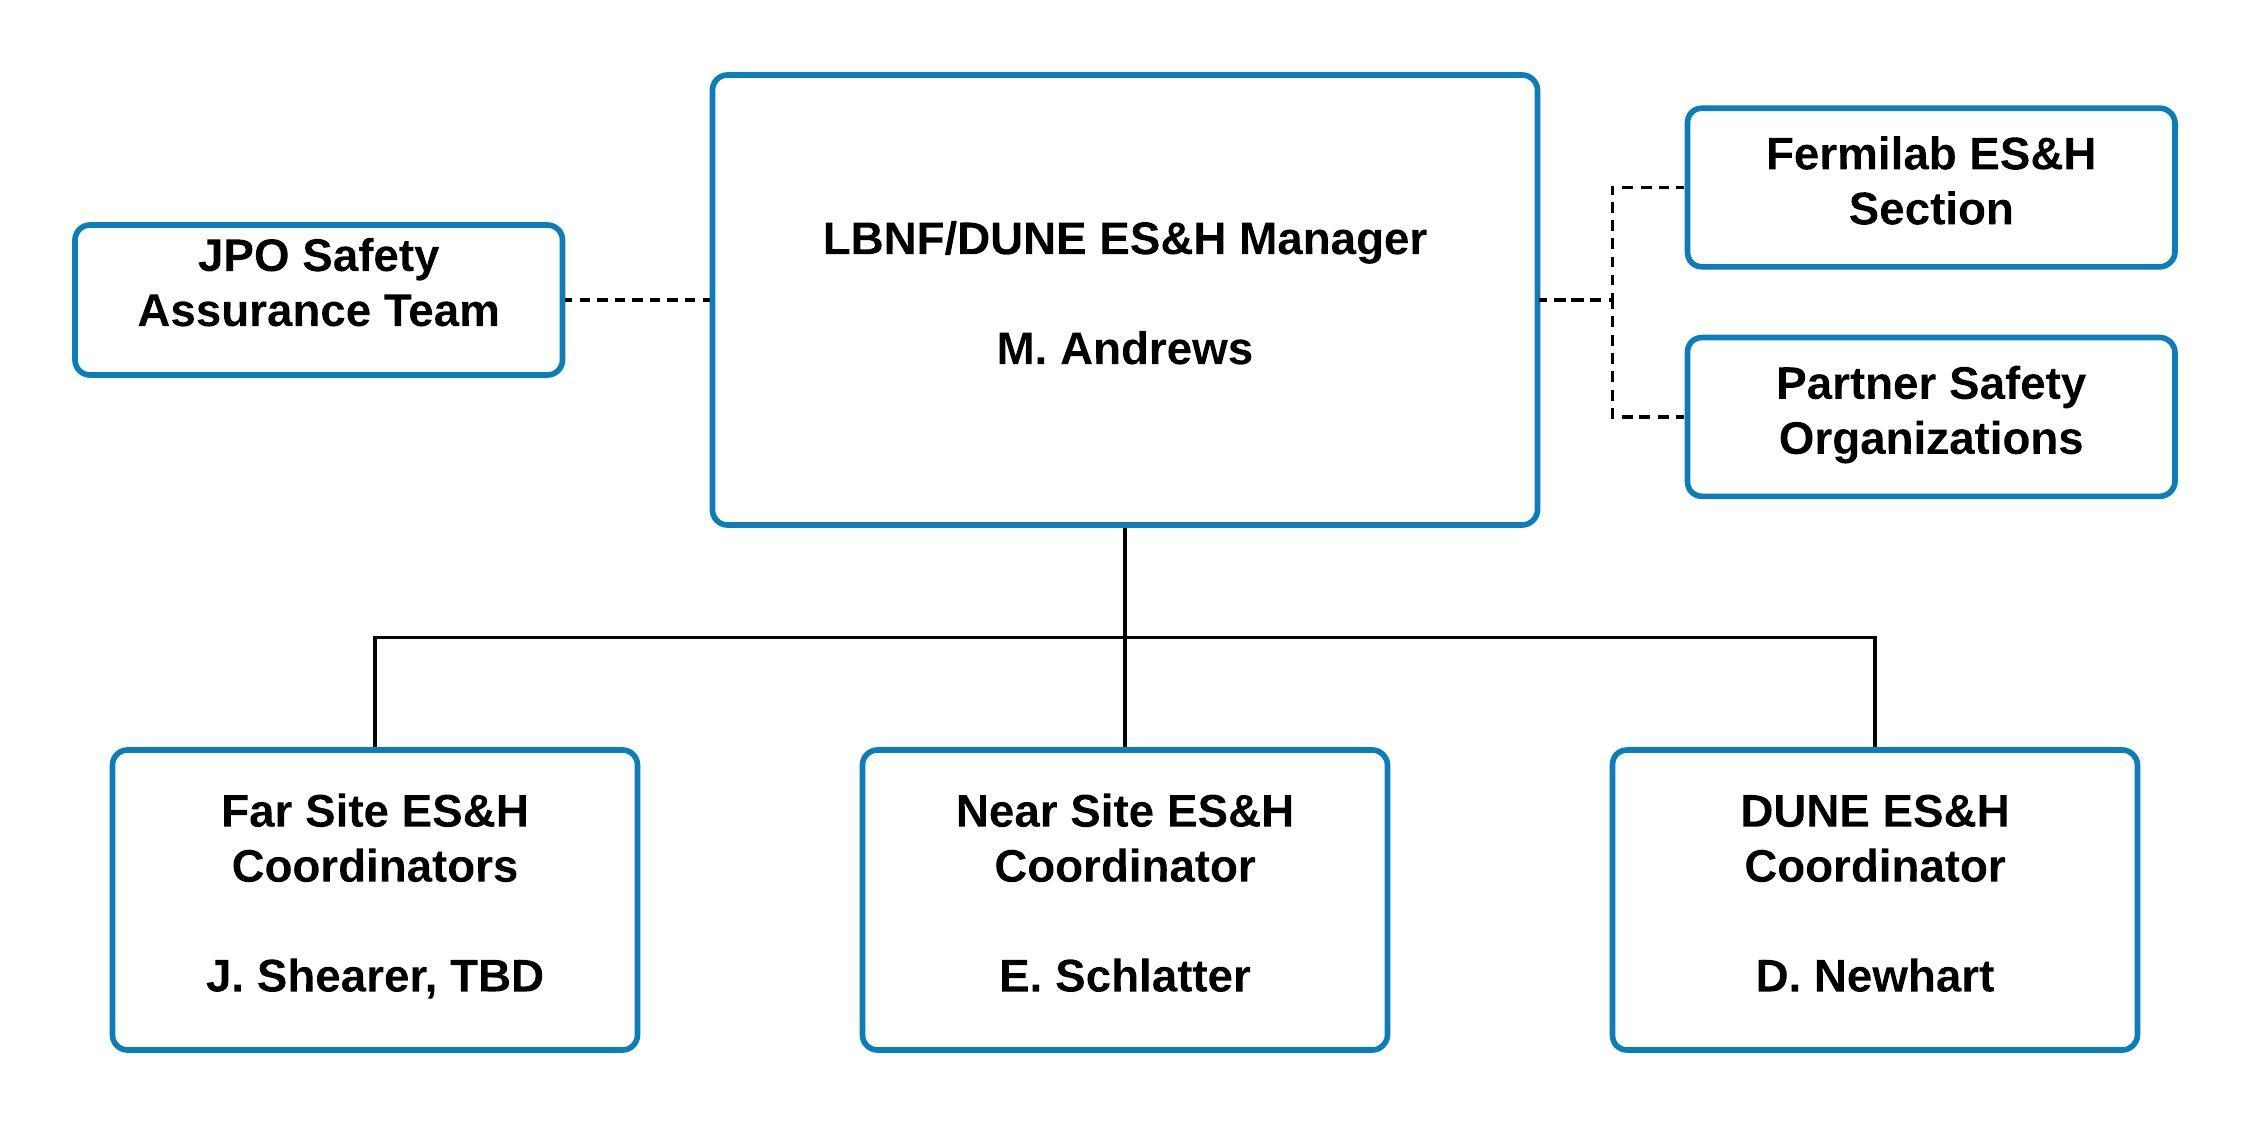
\includegraphics[width=0.85\textwidth]{DUNE_Safety_Org_Chart_v2}
\end{dunefigure}

The project \dword{esh} manager works with a \dword{jpo} 
engineering safety assurance team to ensure consistent application of engineering standards and engineering 
documentation requirements. % across \dword{lbnf-dune}. .

The \dword{jpo} engineering safety assurance team defines a common 
set of design and construction rules (mechanical and electrical) to 
ensure consistent application of engineering standards and engineering 
documentation requirements across \dword{lbnf-dune}. 
Following on lessons learned from the processes used for the 
\dword{protodune} detectors, an important mandate of the engineering 
safety assurance team is to ensure that safety issues related to 
component handling and installation are incorporated within the 
earliest stages of the design review process.


\subsection{Engineering Integration}
\label{sec:dune_engineering}


A central \dword{jpo} engineering team  is responsible for building  
an integrated full \threed CAD model of the detectors within their supporting
infrastructure and the \dword{cf} that house them.  
The \dword{lbnf-dune} project has adopted 
the formal change control process developed previously for the 
\dword{lbnf} project.  The change control process applies to 
proposed changes to requirements, technical designs, 
schedule, overall project scope, and assigned responsibilities 
for individual scope items. 
The \dword{jpo} team incorporates approved design changes as they 
are received and runs a series of checks to ensure that no errors 
or spatial conflicts are introduced into the model. After receiving the 
appropriate sign-offs from all parties, 
The \dword{jpo} team maintains  
each release  of the model and makes it available to the 
design teams as the current release, against which the next set 
of design changes is to be generated. 

Electrical engineers are also incorporated within the central
\dword{jpo} team to properly integrate and install 
the detector electrical components.  

The \dword{jpo} engineering team documents and
controls the interfaces between the \dword{lbnf} and \dword{dune} 
projects as well as the interfaces between these projects and the 
\dword{lbnf}/\dword{dune} integration and installation activities 
at \dword{surf}.  


\subsection{Schedule and Milestones}
\label{sec:dune_schedule}

The \dword{jpo} team also creates a single 
project schedule for \dword{lbnf-dune}, incorporating all 
\dword{lbnf} and \dword{dune} activities with the 
integration and installation activities at \dword{surf} 
as well as all interdependencies.  This schedule will 
be used to track the status of the global enterprise.  
  The non-\dword{doe} activities 
will not be tracked using the formal \dword{evms} procedures 
required for the \dword{doe} project activities but rather 
through management teams responsible for those activities who regularly assess progress toward completion.  


\subsection{Partner Agreements and Financial Reporting}
\label{sec:dune_agreements}

Partner contributions to all project elements will be documented %detailed 
in a series of written agreements.  In the case of \dword{lbnf}, 
these contributions will be spelled out in bilateral agreements 
between \dword{doe} and each of the contributing partners.  In 
the case of \dword{dune}, an \dword{mou} will describe  
%detailing 
the contributions of all participating partners. %\fixme{one mou per contribution or one for all?}
 To accompany these primary agreements, the  \dword{jpo} will coordinate a series of technical agreements, describing the exact 
boundaries between partner contributions and the terms and 
conditions under which contributions will be delivered. 

%%%%%%%%%%%%%%%%%%%%%%%%%%%%%%%%%%%%%%%%%%%%%
\section{Detector Design and Construction Organization}
\label{sec:es-tc-det-const}

The \dword{dune} \dword{fd} construction project refers collectively 
to the activities associated with designing and constructing the
necessary detector components.  \dword{dune} collaboration management 
will oversee this portion of \dword{lbnf-dune} and 
ensure its successful execution.  The high-level \dword{dune} 
collaboration management team, consisting of the co-spokespersons, 
\dword{tcoord}, and \dword{rcoord}, is responsible for day-to-day 
administration of the project.  

Consortia of collaboration institutions, who assume responsibility 
for detector subsystems, construct the \dword{dune} \dwords{detmodule}. Each consortium plans and executes 
construction, installation, and commissioning of its subsystem.  In most cases, a single consortium is responsible for subsystem deliverables supported by 
multiple funding agencies, with each agency managing its own internal projects. 

Each consortium has an overall consortium leader 
and a technical lead.  The consortium leader chairs an institutional 
board comprising one representative from each of the collaborating 
institutions that contribute to the activities of the consortium.  Major 
consortium decisions such as technology selections and assignment of 
responsibilities within the institutions are passed through this institutional 
board.  These decisions are then passed as recommendations to 
the \dword{dune} \dword{exb} for formal collaboration approval.

Because the consortia operate as self-managed entities, a strong
\dword{tc} organization must ensure overall integration 
of the detector elements and successful execution of the detector
construction project.  \dword{tc} areas of responsibility include 
general project oversight, systems engineering, \dword{qa}, and 
safety.  \dword{tc} also supports the planning and execution 
of integration and installation activities at \dword{surf}.  

The \dword{tcoord} manages the overall detector construction project
through regular board meetings with the consortium leadership teams 
and members of the \dword{tc} organization.  
%These board meetings are used to identify and resolve technical issues
%and serve as the primary forums for required interactions between the 
%consortia. Any decisions generated through these board meetings are passed to 
%the \dword{dune} \dword{exb} as recommendations for formal approval.
%
In addition, the \dword{tcoord} heads %an organization 
%a project coordination team 
an organization that supports the work of 
the consortia and has responsibility for a number of major project 
support functions: 
\begin{itemize}
\item ensuring that each consortium has a well defined and complete
  scope, that interactions between consortia are sufficiently 
  well defined, and that any required scope outside the 
  consortia scope is provided through other sources such as collaboration
  common funds;
\item defining and documenting scope boundaries and technical 
  interfaces both between consortia and with \dword{lbnf};  
\item developing an overall schedule with appropriate dependencies
  between activities covering all phases of the project;  
\item ensuring that appropriate engineering and safety standards 
  are developed, understood, and agreed to by all key stakeholders 
  and that these standards are conveyed to and understood by each
  consortium;
\item ensuring that all \dword{dune} requirements on \dword{lbnf} 
  for \dword{cf}, cryostat, and cryogenics are clearly defined and 
  agreed to by each consortium;
\item ensuring that each consortium has well developed and properly reviewed
  component designs, construction plans, \dword{qc} processes, and 
  safety programs; and
\item monitoring the overall project schedule and the progress of 
  each consortium toward delivering its assigned scope. 
\end{itemize}

The \dword{dune} \dword{tc} organizational structure is shown 
in Figure~\ref{fig:DUNE_tc}.  

\begin{dunefigure}[DUNE technical coordination org chart]{fig:DUNE_tc}
  {\dword{dune} \dword{tc} organizational chart.}
  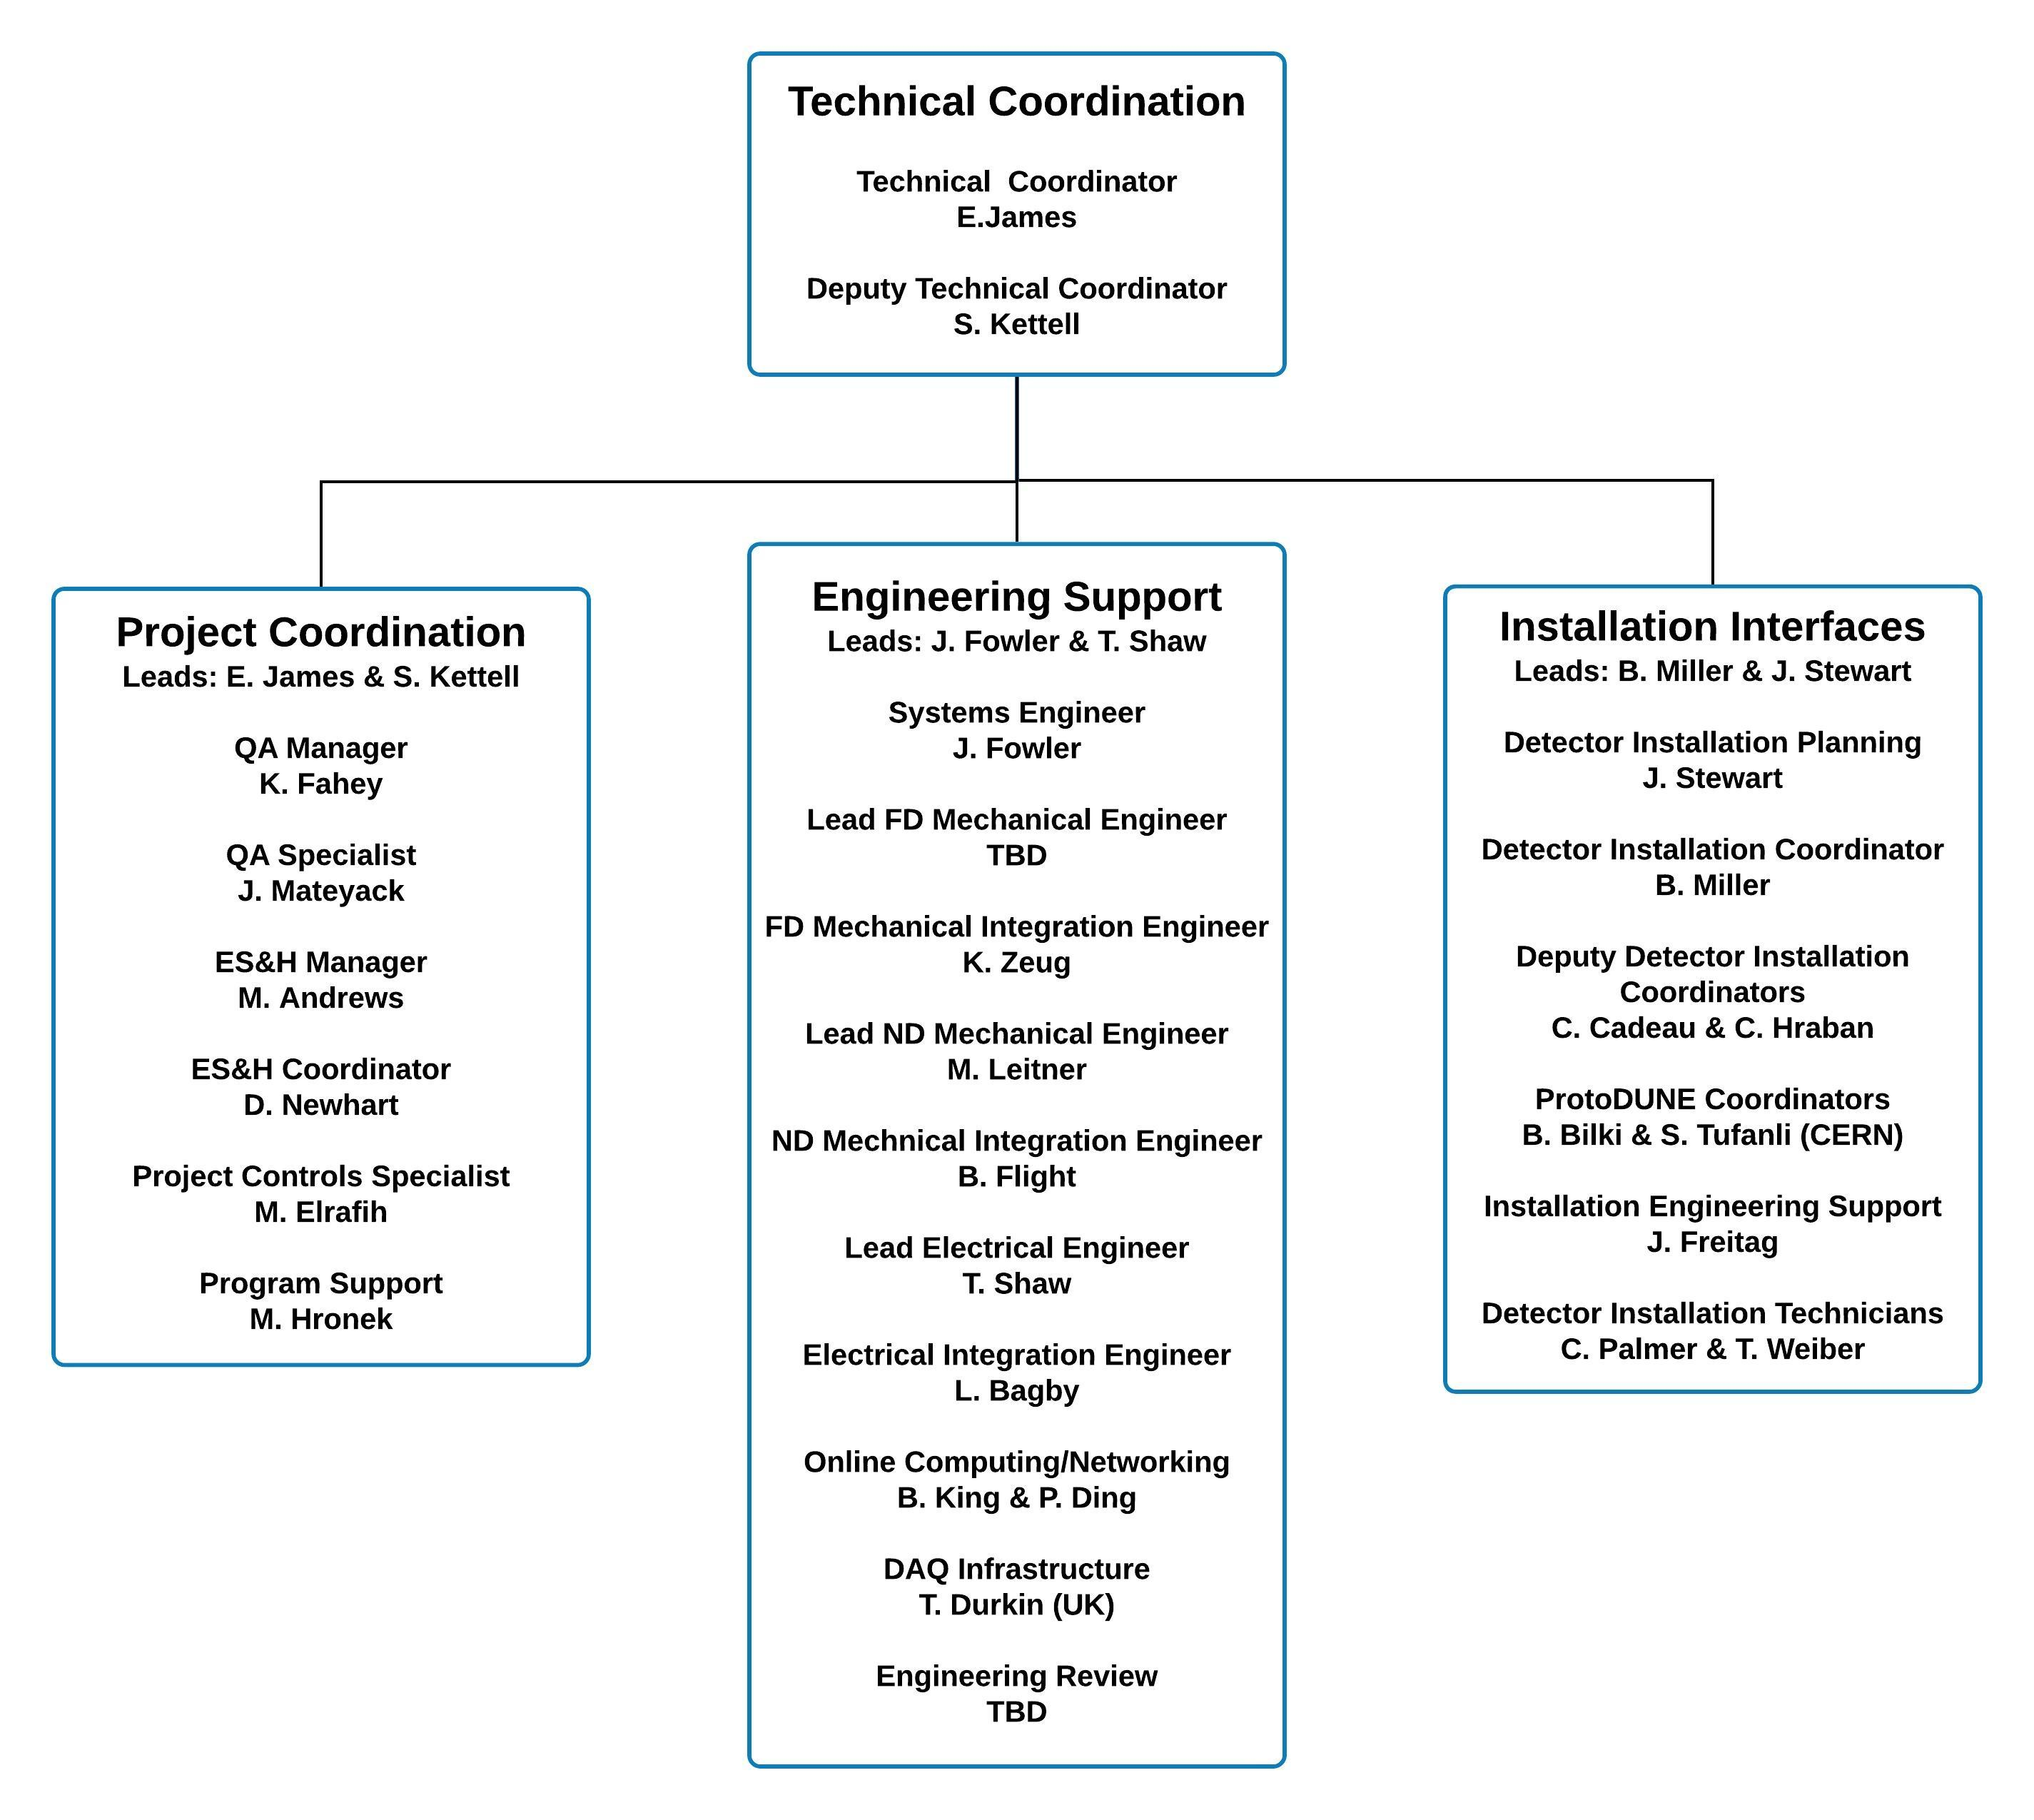
\includegraphics[width=0.99\textwidth]{TC_OrgChart_v2}
\end{dunefigure}

%%
The \dword{tc} project coordination team incorporates \dword{esh}, 
\dword{qa}, and project controls specialists.  Overall integration 
of the detector elements is coordinated through the \dword{tc} 
engineering support team headed by the \dword{lbnf-dune} systems 
engineer and lead \dword{dune} electrical engineer.  Planning 
coordinators for integration and installation activities at 
\dword{surf} sitting within the \dword{lbnf}/\dword{dune} \dword{integoff} also head the \dword{tc} installation interfaces team.  
The dual placement of these individuals facilitates the required 
coordination of integration and installation planning efforts between 
the core team directing these activities and the \dword{dune} 
consortia. 

                                          \begin{comment}  %%%%%%%%%%%%%%%%%%%
The \dword{dune} project has already completed an initial round of design 
and prototyping culminating in the construction and operation 
of the \dword{protodune} detectors.  Moving forward, the project is 
updating detector component designs to incorporate lessons learned from 
the \dword{protodune} experience.  Then the designs are final, the 
project will first construct production versions of all components to be installed and operated in a second phase of \dword{protodune} 
operations before starting full-scale production.  The operation 
of each \dword{protodune2} detector will begin roughly two years after
the end of operations for its corresponding \dword{protodune} detector.
In a few cases, production of components requiring a long lead time must 
be started in parallel with the operation of first production components 
in \dword{protodune2}.
                                          \end{comment}  %%%%%%%%%%%%%%%%%%%

%%%%%%%%%%%%%%%%%%%%%%%%%%%%%%%%%%%%%%%%%%%%%
\section{Detector Installation and Commissioning Organization}
\label{sec:es-tc-det-instal}

The \dword{ipd} has
responsibility for coordinating the planning and execution of 
the \dword{lbnf-dune} installation activities, both 
in the underground detector caverns at \dword{surf} and in 
nearby surface facilities. The coordinators of this activity and crucial technical support
staff sit within the \dword{integoff}.
The \dword{lbnf-dune} \dword{integoff} will evolve over 
time to incorporate the team in South Dakota responsible for the 
overall coordination of onsite installation activities.  In the 
meantime, the installation planning team within the \dword{integoff} works with 
the \dword{dune} consortia and \dword{lbnf} project team members 
to plan these activities.  This team is responsible for specification 
and procurement of common infrastructure items associated with 
installation of the detectors. The organization of this onsite team is 
shown in Figure~\ref{fig:io-org-chart}.

\begin{dunefigure}[\dshort{lbnf-dune} IO organization chart]{fig:io-org-chart}
  {\dword{lbnf-dune} \dword{integoff} organization chart}
  \includegraphics[width=0.95\textwidth]{Org-Far-Site-TDR-10-9-19}
\end{dunefigure}

The onsite \dword{integoff} team includes rigging teams responsible for moving 
materials in and out of the shaft, through the underground drifts, 
and within the detector caverns, and personnel responsible 
for overseeing safety and logistics planning.  

The onsite safety organization, including the far site \dword{esh} coordinators
working under the direction of the \dword{lbnf-dune} \dword{esh}
manager, oversee all onsite activites and have a %direct 
reporting line to the \dword{ipd}.

%%%%%%%%%%%%%%%%%%%%%%%%%%%%%%%%%%%%%%%%%%%%%
\section{Facility Description}
\label{sec:es-tc-facility}

The \dword{dune} underground campus at the \dword{surf} 4850L is shown in
Figure~\ref{fig:dune-underground}. The primary path for both personnel 
and material access to the underground excavations is through the Ross Shaft.
\begin{dunefigure}[Underground campus]{fig:dune-underground}
  {Underground campus at the 4850L.}
  \includegraphics[width=0.75\textwidth]{underground_campus_vertical}
\end{dunefigure}

\dword{lbnf} will provide facilities and services, on the surface and
underground, to support the \dword{dune} detectors.  This includes
logistical, cryogenic, electrical, mechanical, cyber and environmental
facilities and services.  All of these facilities are provided for the
safe and productive operation of the \dwords{detmodule}.

On the surface, a new compressor building will house the cryogenics
systems for receiving cryogenic fluids and preparing them for delivery
down the Ross Shaft.  New transformers are being installed in the Ross substation to support the underground power needs, and new power cables are
being installed down the Ross Shaft to transmit the power underground
to a new substation.  A portion of the Ross Dry basement will house the
surface cyber infrastructure.


Two large underground detector caverns
are being excavated.  Each of these caverns will support two
\SI{17}{\kilo\tonne} cryostats and the required infrastructure.  These caverns are \SI{144.5}{\meter} long, \SI{19.8}{\meter} wide and
\SI{28.0}{\meter} high. The tops of the cryostats are approximately
aligned with the 4850L with the cryostats resting
at the 4910L.  A \SI{12}{\meter} space between the cryostats will
be used as part of the detector installation process, placement of
cryogenic pumps and valves, and for access to the 4910L.  A
\dword{cuc}, between the detector caverns, is \SI{190}{\meter}
long, \SI{19.3}{\meter} wide, and \SI{10.95}{\meter} high.

Laydown space near the Ross Headframe is extremely 
limited, therefore  no materials or equipment can be shipped directly to \dword{surf}. The \dword{sdwf} will be a leased 5000m$^2$ facility, hosted by 
\dword{sdsd}, to be used for both short- and long-term storage, as 
well as for any re-packaging of items required prior to transport 
into the underground areas.  It must be in place approximately six months before \dword{aup}
of the underground detector caverns is received.  

%%%%%%%%%%%%%%%%%%%%%%%%%%%%%%%%%%%%%%%%%%%%%
\section{DUNE Detector Construction Management}
\label{sec:es-tc-det-mgmt}

%\fixme{I think this should be melded with section \ref{sec:es-tc-det-instal} - two sections back. anne}

A total of eleven \dword{fd} consortia have been formed to cover 
the subsystems required for the two detector types currently under
consideration.  In particular, three consortia (SP-APA, SP-TPC
Electronics and SP-Photon Detection) pursue subsystems specific to
the single-phase design and another three consortia (DP-CRP, DP-TPC
Electronics and DP-Photon Detection) pursue designs for \dword{dp}
specific subsystems.  An additional five consortia (HV System, \dword{daq},
Cryogenic Instrumentation/Slow Controls, Calibration, and Computing)
have responsibility for subsystems common to both detector
technologies.  Figure~\ref{fig:DUNE_consortia} shows the consortia 
associated with the \dword{fd} construction effort along with their 
current leadership teams.  
\begin{dunefigure}[DUNE consortia]{fig:DUNE_consortia}
  {\dword{dune} consortia organization. CL refers to consortium leader
    and TL refers to technical lead.}
  \includegraphics[width=0.99\textwidth]{Consortia_Org_Chart}
\end{dunefigure}

The complete scope of the \dword{dune} construction project is captured in a 
\dword{wbs} to understand the distribution of deliverables between 
the consortia.  In combination with interface documentation, the 
\dword{wbs} is used to validate that all necessary scope is covered.  The 
\dword{wbs} is also used as a framework for building \dword{dune} 
detector cost estimates. 

The highest-level layers of the \dword{dune} \dword{wbs} are summarized 
in Figure~\ref{fig:WBS_level2}.  At Level-1 the \dword{wbs} is broken down into 
six elements corresponding to the five \dword{dune} detector modules (four 
\dword{fd} and one \dword{nd}) and \dword{tc}.  The scope documented
here is fully contained within the \dword{tc}, first \dword{fd} module 
(\dword{sp}), and second \dword{fd} module (\dword{dp}) Level-1 elements.   
\begin{dunefigure}[DUNE WBS at level-2]{fig:WBS_level2}
  {High level \dword{dune} \dword{wbs} to level-2.}
  \includegraphics[width=0.75\textwidth]{WBS_level2_v2}
\end{dunefigure}

The underground cavern coordinator is responsible for managing all 
activities in the two undergound detector caverns as well as the
\dword{cuc}. The detector
installation teams incoporate a substantial number of scientific and
technical personnel from the \dword{dune} consortia.  \dword{integoff} coordinators 
of the detector installation effort are jointly placed within 
\dword{dune} \dword{tc} to facilitate consortia involvement in the 
detector installation activities.  Any modifications to the facilities 
occuring after \dword{aup} are managed by the underground cavern 
coordinator under the direction of the \dword{ipd}.

The team responsible for detector installation incorporates 
members of the technical support team described above 
and includes scientific and technical personnel from 
the \dword{dune} consortia.  The team is led by the detector
installation manager who has three shift supervisors working 
with them to provide onsite coverage for every shift.
The management team works with the underground cavern
coordinator to ensure that required technical support team 
members are available as needed and that required materials 
are delivered to the detector caverns on a schedule to keep
the installation effort moving forward.   

%%%%%%%%%%%%%%%%%%%%%%%%%%%%%%%%%%%%%%%%%%%%%
\section{Integration Engineering}
\label{sec:es-coord-integ-sysengr}

Integration engineering for \dword{dune} focuses on configuring the
mechanical and electrical systems of each \dword{detmodule} and managing
the interfaces within them. This includes verifying that subassemblies
and their interfaces are built conforming to the approved design,
e.g., \dword{apa} or \dword{pds}. The second major focus
is assuring that the \dwords{detmodule} can be integrated and
installed into their final configuration. And the third major focus is
integrating necessary services provided by \dword{cf} 
with the \dwords{detmodule}.

To this end, the \dword{jpo}/\dword{tc} engineering team maintains
subsystem component documentation in order to manage the detector
configuration. The consortia provide engineering data for their
subsystems to \dword{tc}. The \dword{jpo}/\dword{tc} engineering team
works with the \dword{lbnf} project team and \dword{jpo} to integrate
all detector data into the global \dword{lbnf} configuration files.

\subsection{Mechanical Integration Models}
\label{sec:es-tc-mech}

%\fixme{I didn't update anything here - it seems ok still relative to the TC vol. Anne}

Three dimensional (\threed) mechanical modeling techniques can represent the \dwords{detmodule} well and manage their configurations, but because  \threed modelling techniques vary, a set
of clear and unambiguous \twod integration drawings must first be generated to serve as
the basis for the \threed model accuracy and for the engineering
design of all components. The \twod integration drawings must show the 
interfaces to the level of detail necessary to ensure proper fit and function.  These \threed and 
\twod models are considered static because they do not represent effects of gravity, tolerances, cold
temperature, and installation and assembly clearances.

For installation and operation, however, envelope models  are developed to 
show the effects on the detector 
caused by, among others, distortion of the cryostat and \dword{dss} due to gravity, loads  during 
detector filling and operation, thermal contraction,  as well as tolerances and clearances for tooling.

Interfaces among components are developed, managed, and controlled through additional models and drawings. 
Integration drawings are derived directly from the overall
integration model, which in turn is assembled from
component models developed by the consortia.
\dword{tc} is responsible for controlling many of these interfaces. 

\subsection{Electrical Integration}
\label{sec:es-tc-elec}

\dword{tc} is responsible for the \dword{ac} power
distribution supplied to the experiment and to detector electronics
racks.  Through the design review process, \dword{tc} will  ensure 
that all electrical systems  follow safe design practices and
will pass \dwords{orr}. We will follow the same  guidelines\cite{bib:cernedms2095958} for \dword{dc} power supplies as
were followed at \dword{protodune} and developed during extensive testing of
the \dword{apa} wire readout at \dword{bnl} and \dword{protodune}.  

The electrical design of each subsystem is described by a set of
documents that includes a system-level block diagram and a wiring
diagram that includes a complete description of all power and ground
connections.  Depending on what is being described, a complete set of
schematics, board production files and wiring diagrams will be
reviewed and archived.  All designs are subject to electrical safety
review, as described above, before production proceeds. 

The \dword{tc} team will provide unique names and labels
for all racks, crates, boards, power supplies, cables, and any other
electrical type equipment.  A database will be created to track these
devices.

\subsection{Configuration and Drawing Storage and Dissemination}
\subsection{Organization of Interfaces and Interface Documents}

The consortia and \dword{jpo}/\dword{tc} engineering team create and share
drawings, models, schematics, production data and all other
engineering documents. In addition, the \dword{jpo}/\dword{tc} engineering team
generates and shares all interface drawings and documentation.

\subsection{Integration}
\label{sec:es-tc-integ}

 An integration mechanism has been developed to manage and create an overall model of interfaces both within a \dword{detmodule} and between a \dword{detmodule} and facilities.
 The \dword{jpo} engineering team carries out  and manages interfaces between the nodes.

\begin{dunefigure}[Integration Nodes]{fig:integration_nodes}
  {Overall integration nodes and interfaces.}
  \includegraphics[width=0.7\textwidth]{Integration_nodes.png}
\end{dunefigure}

Figure~\ref{fig:integration_nodes} shows the interfaces between the
detector and facilities. In this figure, within the cavern, items
provided by \dword{lbnf} are on the left and the items provided by
\dword{dune} are on the right. 
In addition, the \dword{jpo}/\dword{tc} engineering
team integrates (ensures that the interfaces are appropriately defined
and managed) the \dword{daq} room in the \dword{cuc} and surface
control and network rooms. Interfaces with \dword{lbnf}
are managed at the boundaries of each integration node. 
Interface documents are developed and maintained to manage the
interfaces between consortia and between each consortium and the
\dword{tcoord}.

\subsection{Engineering Change Control}

Changes in design and fabrication requirements follow revision
processes for design and fabrication documents, per individual
consortium practice, while ensuring appropriate levels of
verification, review and approval by the consortium design authority.

\subsection{Value Engineering}
\label{sec:es-tc-fdsp-coord-ve}

Value engineering is the process of arriving at cost-effective
solutions to the technical challenges of building the \dword{dune}
detector. \dword{dune} value engineering builds on significant
developments in \dword{lar} detectors,  
especially the large \dwords{lartpc} \dword{icarus} and
\dword{microboone}. Prototypes up to and including the \dword{protodune} 
detectors have been used to validate
\dword{dune} designs and confirm that the necessary performance is
met.

Value engineering is ongoing at all stages of design and will continue
through fabrication, assembly, and installation phases. In
particular, during the fabrication and assembly stages, when labor costs
are relatively higher, this can result in significant cost savings.  The
consortia and \dword{jpo}/\dword{tc} are actively engaged and have the necessary
experience for this ongoing process.

%%%%%%%%%%%%%%%%%%%%%%%%%%%%%%%%%%%%%%%%%%%%%
\section{Reviews}
\label{sec:es-tc-reviews}

\fixme{Review office or review team - or whatever Eric had...? anne}
The \dword{jpo} \dword{dune} Review Office reviews all stages of
detector development and works with each consortium to arrange reviews
of the design (\dword{cdrev}, \dword{pdr} and \dword{fdr}), production
(\dword{prr} and \dword{ppr}) and \dword{orr} of their system. These
reviews provide information to the \dword{tb} to help in evaluating
technical decisions.  Review reports are tracked by \dword{tc} and
provide guidance on the key issues that require engineering oversight
by the \dword{tc} engineering team. In parallel the Reciew office
reviews all stages of \dword{lbnf} cryostat and cryogenics
development. The Review Office maintains a calendar of \dword{dune}
reviews.


Production of detector elements begins only after successful
\dwords{prr}. Regular production progress reviews will be held once
production starts. 

The review process is an important part of the \dword{dune} \dword{qa}
process for design and production.

%%%%%%%%%%%%%%%%%%%%%%%%%%%%%%%%%%%%%%%%%%%%%
\section{Quality Assurance}
\label{sec:es-tc-qa}

The primary objective of the \dword{lbnf-dune} \dword{qa} program is
to assure quality in the construction of the \dword{lbnf} facility and
\dword{dune} experiment while protecting
\dword{lbnf-dune} personnel, the public, and the environment. The
\dword{qa} plan aligns \dword{lbnf-dune} \dword{qa} activities, which
are spread around the world, with the principles of the \fnal Quality
Assurance Manual. The manual identifies the \fnal Integrated Quality
Assurance Program features that serve as the basis for the
\dword{lbnf-dune} \dword{qa} plan.

The \dword{lbnf-dune} \dword{qa} plan incorporates 
a graded approach; it applies a level of analysis,
controls, and documentation commensurate with the potential for any effect on
environment, safety, health, or quality.

One part of the \dword{tc}'s centralized project
coordination functions is
standardizing \dfirst{qa}/\dfirst{qc} practices, one facet
of which is to assist consortia in defining and implementing
\dword{qa}/\dword{qc} plans that maintain uniform high
standards across the entire detector construction
effort. Figure~\ref{fig:fnal_qa} shows how \dword{dune} \dword{tc}
derives its \dword{qa} program from the principles of the \fnal \dword{qa} program:
requirements are flowed down through the \dword{lbnf-dune}
\dword{qa} program into the \dword{qc} plans developed for consortia fabricating detector components and integrating and installing the detector.

\begin{dunefigure}[\fnal QA]{fig:fnal_qa}
  {Flow-down of \fnal \dword{qa} to consortia.}
  \includegraphics[width=0.85\textwidth]{fnal_qa.pdf}
\end{dunefigure}

The \dword{qa} effort includes design, production readiness, and
progress reviews as appropriate for the \dword{dune} detector
subsystems, as was done for \dword{pdsp} under \dword{tc}
oversight. Continuous improvement through documentation of lessons learned and best practices is
an integral part of the program. 


The \dword{dune} consortium leaders identify the
resources to ensure that their team members are adequately trained and
qualified to perform their assigned work. 
All consortium members, in turn, are responsible for the quality of the work that
they do and for using available guidance and assistance. All members 
have the authority to stop work and report adverse conditions that
affect the quality of \dword{dune} products to their 
\dword{dune} consortium leader and the \dword{lbnf-dune}
\dword{qa} manager. The \dword{qa} plan
defines the \dword{qa} roles and responsibilities within the \dword{dune}
project.


%%%%%%%%%%%%%%%%%%%%%%%%%%%%%%%%%%%%%%%%%%%%%
\section{Environment, Safety, and Health}
\label{sec:es-tc-eshq}

\subsection{LBNF-DUNE ES\&H Management and Oversight}
\label{sec:es-tc-eshq-prog}

\dword{lbnf-dune} is committed to protecting the health and
safety of staff, the community, and the environment, as stated in the
\dword{lbnf-dune} integrated \dword{esh} plan.  
The \dword{lbnf-dune} \dword{esh} program complies with applicable
standards and local, state, federal and international legal
requirements through the \fnal work smart set of standards and the
contract between Fermi Research Alliance (FRA) and the \dword{doe}
Office of Science (FRA-DOE). \fnal, as the host laboratory,
established the \dword{sdsd} to provide facility support.
\dword{sdsd} is responsible for support of \dword{lbnf-dune}
operations at \dword{surf}.


The \dword{lbnf-dune} \dword{esh} management system is
designed to work hand-in-hand with the \dword{surf} emergency
management systems to protect the public, workers, and the environment;
ensure compliance with the FRA-\dword{doe} contract and \fnal Work Smart
standards; and improve the \dword{dune} ability to meet or
exceed stakeholder expectations and execute the
scientific mission.  \dword{dune} uses a set of criteria to plan, direct,
control, coordinate, assure, and improve how \dword{esh} policies,
objectives, processes, and procedures are established, implemented,
monitored and achieved.




The \dword{tcoord} and \dword{ipd} are responsible for
implementing the \dword{dune} \dword{esh} program.  The
\dword{lbnf-dune} \dword{esh} manager reports  to the
\dword{tcoord} and \dword{ipd} and provides
\dword{esh} support and oversight for developing and implementing the
\dword{lbnf-dune} \dword{esh} program. The \dword{dune} \dword{esh}
coordinator reports to the \dword{lbnf-dune} \dword{esh}
manager and has primary responsibility for \dword{esh} support and
oversight of the \dword{dune} \dword{esh} program for all activities
at collaborating institutions. % and at \dword{lbnf-dune} facilities located at \dword{surf}. 
The far and near site \dword{esh} coordinators are responsible for providing 
daily field support and
oversight for all installation activities at the \dword{surf}
and \dword{fnal} sites. 
The \dword{lbnf-dune} \dword{esh} plan defines the \dword{esh}
requirements applicable to installation activities at \dword{surf}. 

The \fnal \dword{esh} Section, \dword{doe}, and
\dword{lbnf} \dword{esh} have completed a series of assessments of
critical \dword{sdsta} \dword{esh} programs including underground access,
emergency management, electrical safety, rigging, and fire
protection. The findings and lessons learned identified in these
\dword{esh} program assessments are tracked within the \fnal issues management
database --- iTrack.
%It tracks the findings and lessons learned identified in these and other reviews and assessments, disseminate them where applicable, and ensure they are appropriately implemented.

\subsection{National Environmental Protection Act Compliance}  

In compliance with the National Environmental Protection Act and in
accordance with \dword{doe} Policy 451.1, the
\dword{lbnf-dune} project performed an evaluation of potential
environmental impacts during construction and operation of the
project.  An environmental assessment %has been prepared on 
of the potential environmental impacts and the safety and health hazards
identified during the design, construction, and operating phases of
\dword{lbnf-dune} was completed, and
a finding of no significant impact (FONSI) was issued in September 2015.


%\subsection{Hazard Identification} 
\begin{comment}
\subsection{Work Planning and Controls}
\label{sec:es-tc-eshq-har}
\fixme{ this was titled `Hazard Identification,' but has this other title in TC vol}

\fixme{I'm not sure what you want here; I mostly left the old text. anne}
A key element of an effective \dword{esh} program is identifying hazards. All work activities
shall be subject to work planning and hazard analysis.  
Once a list of hazards has been compiled for a facility, these hazards can be screened
and managed through a suitable set of controls.

The \dword{lbnf-dune} project completed a Hazard Analysis Report (\dword{har})
to ensure that identified hazards are mitigated early in the
design process.  The focus of the report is process hazards,
not activity hazards, which are typically covered in a job hazard
analysis.  The \dword{har}  identifies
hazards anticipated in the project's construction and operational
phases, proposes ways to mitigate the hazards to reduce risk, and establishes a
post-mitigation risk category for each.  As the \dword{dune} design 
matures, the \dword{har} will be
updated to ensure that all hazards are properly identified and
controlled through design and safety management programs.
\end{comment}

\subsection{Codes/Standards Equivalencies}
\label{sec:es-tc-esh_codes}

\dword{dune} will rely on significant contributions from international
partners. In many cases, an international partner will contribute
equipment for installation at \dword{fnal} or \dword{surf} built
following international standards. \dword{fnal} has established a
process under the international agreement with \dword{cern}, detailed
in \dword{feshm} Chapter 2110, to establish code equivalency between
USA and international engineering design codes and standards. This
process allows the laboratory to accept in-kind contributions from
international partners or purchase equipment designed using
international standards while ensuring an equivalent level
of safety.



\subsection{ES\&H Requirements at Collaborating Laboratories and Institutions}

All work performed at collaborating institutions will be completed
following that institution's \dword{esh} policies and
programs. Equipment and operating procedures provided by the
collaborating institution will conform to the \dword{dune} project
\dword{esh} and integrated safety management policies and
procedures. The \dword{esh} organization at collaborating institutions
provides \dword{esh} oversight for work activities carried
out at their facilities.

\subsection{\dshort{lbnf-dune} \dshort{esh} Program at \dshort{surf}}

All \dword{dune} workers requiring access to the \dword{surf} site
register through the \fnal Global Services Office to receive the
necessary user training and a \fnal identification number that can be
used to apply for a \dword{surf} identification badge, through the
\dword{surf} Administrative Services Office. This is coordinated by
\dword{sdsd}. 

\dword{surf} underground access will require that working groups
obtain a \dword{tap} for each daily access to the
underground areas and all personnel are required to ``brass in and
out'' at the entrance to the Ross Shaft
cage prior to accessing the underground facilities.
 Personnel shall wear the required \dword{ppe} when on site at \dword{surf}. 
A detailed list of the \dword{ppe} appears in \tcchesh. 


Each \dword{dune} collaborator, as part of registration through the \fnal Global Services Office,
will complete the user \dword{esh} training modules, and the supervisor
will complete a training needs assessment to develop a training plan
to define additional \dword{dune} \dword{esh} training requirements for the collaborator.
In addition, all personnel performing work onsite at \dword{surf} must
attend \dword{surf} \dword{esh} Site Orientation before beginning work at the site.
\begin{comment}
All work activities
shall be subject to work planning and hazard analysis. 
Work planning ensures the scope of
the job is understood, appropriate materials are available, all
hazards have been identified, mitigation efforts established, and all
affected employees understand what is expected of them.   
All work planning documentation will be reviewed and
approved by the \dword{dune} \dword{esh} coordinator and the \dword{dune}
\dword{esh} review committee before beginning work activities.

A safety data sheet must be supplied for all chemicals and
hazardous materials used on site. All chemicals and hazardous
materials brought to the \dword{surf} site must be reviewed/approved by the
\dword{dune} \dword{esh} coordinator and the \dword{surf} \dword{esh}
department before arriving on site.

An emergency management program will be in place that incorporates an \dword{ert},  trained guides on all underground levels during all shifts, and protocols for treating injuries, accidents, or spills.

Fire and life safety requirements for \dword{lbnf-dune} areas
were analyzed in the \dword{lbnf-dune} Far Site Fire and Life
Safety Assessment. All caverns will be equipped with fire detection
and suppression systems with both visual and auditory notification.  
\dword{surf} will monitor all fire alarms and system supervisory signals, and the \dword{surf} \dword{ert}. 
will respond to the signals, with additional support from the local Lead-Deadwood Fire
Department as needed.  The caverns will also be equipped
with an \dword{odh} monitoring and alarm system with independent visual and
auditory notification systems.


All workers on the \dword{dune} project have the
authority to stop work in any situation that presents an imminent
threat to safety, health, and the environment. Work may not resume
until the circumstances are investigated and deficiencies corrected,
including the concurrence of the \dword{dune} \dword{ipd}
and the \dword{lbnf-dune} \dword{esh} manager.
\end{comment}

